\section{Simulation of Price Distribution}
\label{sec:simulation}

\begin{frame}{Simulation of Price Distribution}{Prediction Framework}
  \begin{enumerate}
  \item<2-> Draw \(N\) samples, \(u_{n,h}\) from the vine copula model, which will be an \(N \times 24\) matrix, uniformly distributed (column-wise)
  \item<3-> Transform each column with the estimated quantile function for the residuals of the ARMA-GARCH models, producing \(t\)- or skew-\(t\)-distributed draws, \(z_{n,h}\)
  \item<4-> Use tail of input values for the ARMA-GARCH models together with \(z_{n,h}\) to calculate \(X_{n,h}\)
  \item<5-> Calculate \(s_{n,h}\) and add to \(X_{n,h}\) to obtain \(p_{n,h}\)
  \item<6-> Prices in EUR/MW are then \(P_{n,h} = \exp p_{n,h} - K\)
  \end{enumerate}
\end{frame}

\begin{frame}{Simulation of Price Distribution}{Example}
  \begin{block}{Predicting the payoff distribution of a forward contract}
    Let \(F\of{t, t_{1}, t_{2}}\) be a price in EUR/MW determined today (at time \(t\)) for delivery of power in the period \(\intcc{t_{1}, t_{2}}\).
    Payoff on a long position is then
    \begin{equation*}
      \sum_{s=t_{1}}^{t_{2}} \sum_{h\in H(s)} \del{P_{s,h} - F\of{t, t_{1}, t_{2}}},
    \end{equation*}
    where \(H(s) \subseteq \cbr{1,\dotsc,24}\) are the hours on day \(s\) for which the forward is in effect.
  \end{block}
\end{frame}

\begin{frame}{Simulation of Price Distribution}{Example}
  \begin{block}{Example simulation}
    \begin{enumerate}
    \item Prices simulated for the period 2019-01-01 -- 2019-07-31

      \(\implies\) 212 observations \(\times\) 24 hours.
    \item Payoff calculated for some contract \(F\of{t, t_{1}, t_{2}}\)
    \item Steps 1--2 repeated 500 times

      \(\implies\) simulated payoff distribution
    \end{enumerate}
   \end{block}
   \begin{block}{}<2->
     For example, if the delivery interval is February 2019, on hours 2--4 and 16--18, for 40 EUR/MW, the simulated mean payoff is \textbf{14.10}, while the payoff using actual prices is \textbf{5.05}.
   \end{block}
\end{frame}

\begin{frame}{Simulation of Price Distribution}{Example}
  \begin{center}
    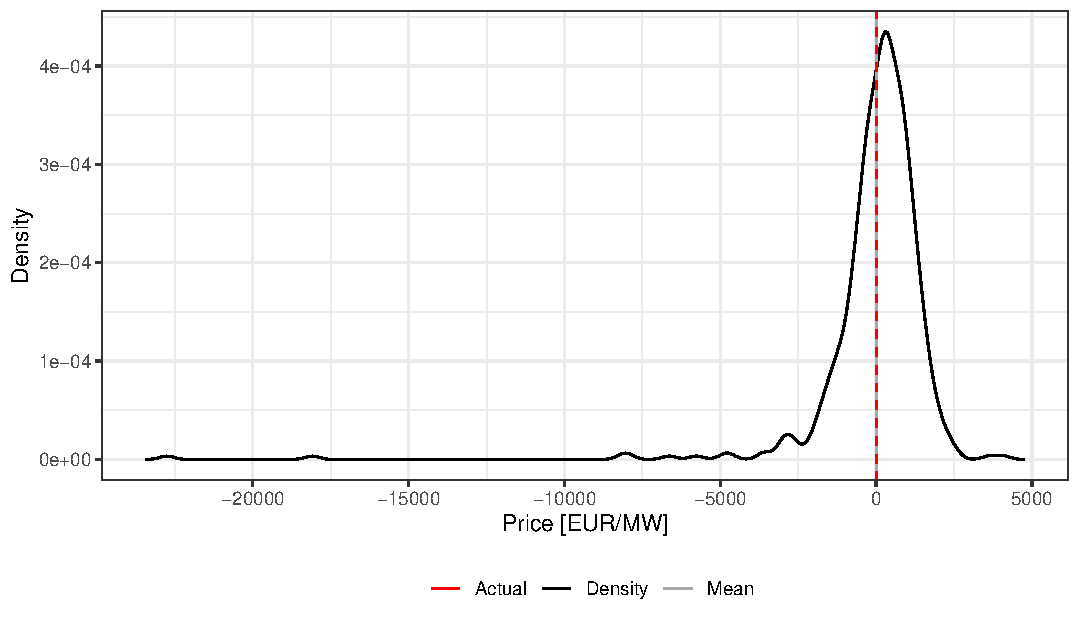
\includegraphics[width=\textwidth]{img/payoff-density}
  \end{center}
\end{frame}

\begin{frame}{Simulation of Price Distribution}{Example of Single Draw}
  \begin{center}
    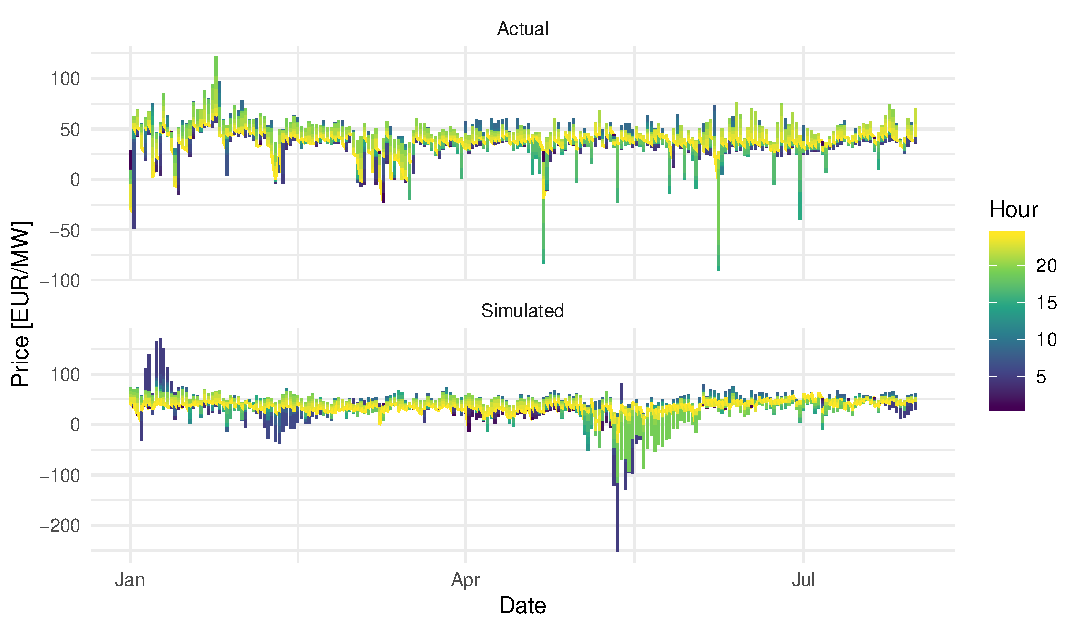
\includegraphics[width=\textwidth]{img/sim-vs-actual}
  \end{center}
\end{frame}

%%% Local Variables:
%%% mode: latex
%%% TeX-master: "../slides"
%%% End:
